\documentclass[tikz,border=4pt]{standalone}
\usepackage[T1]{fontenc}
\usepackage{tikz}
\usetikzlibrary{arrows.meta,positioning,fit,backgrounds,calc,shapes.geometric}

\definecolor{atlasblue}{HTML}{2F6DB2}
\definecolor{atlasgreen}{HTML}{2E8B57}
\definecolor{atlasorange}{HTML}{C86B1F}
\definecolor{atlaspurple}{HTML}{7A3DB8}
\definecolor{atlasink}{HTML}{2F3440}
\definecolor{atlasgray}{HTML}{EEF2F6}
\definecolor{atlasline}{HTML}{667085}

\tikzset{
  phasepanel/.style={
    draw=#1!75!black,
    fill=#1!7,
    rounded corners=4pt,
    line width=0.9pt
  },
  phasehead/.style={
    draw=#1!75!black,
    fill=#1!18,
    rounded corners=3pt,
    minimum width=53mm,
    minimum height=8mm,
    align=center,
    font=\bfseries\footnotesize,
    text=#1!55!black
  },
  mini/.style 2 args={
    draw=#1!70!black,
    fill=white,
    rounded corners=2.5pt,
    minimum width=#2,
    minimum height=6.6mm,
    align=center,
    font=\scriptsize,
    line width=0.8pt
  },
  dotlabel/.style={font=\scriptsize\bfseries,text=atlasink},
  arrow/.style={-{Stealth[length=3mm,width=2.2mm]},line width=0.85pt,color=atlasline},
  softarrow/.style={-{Stealth[length=2.7mm,width=2mm]},line width=0.75pt,color=atlasline,dashed},
  client/.style={draw=#1!75!black,fill=#1!12,rounded corners=2pt,minimum width=10.5mm,minimum height=5.5mm,font=\tiny,line width=0.65pt,align=center},
  circleicon/.style={circle,draw=#1!70!black,fill=#1!12,minimum size=5.6mm,line width=0.75pt,font=\tiny\bfseries,text=#1!60!black},
  rankchip/.style={draw=#1!70!black,fill=#1!12,rounded corners=2pt,minimum width=9mm,minimum height=5mm,font=\tiny,line width=0.65pt},
  ellipsis/.style={font=\large\bfseries,text=atlasink}
}

\begin{document}
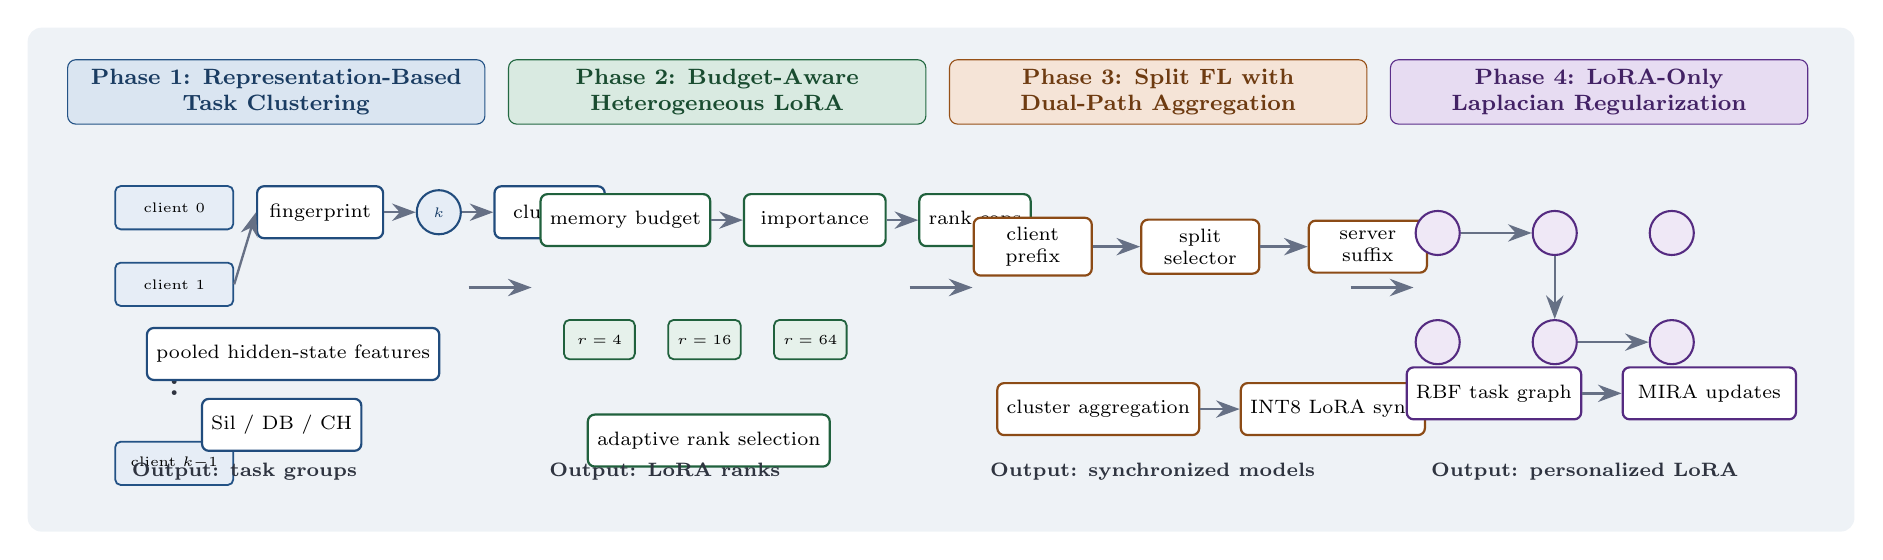
\begin{tikzpicture}[x=1mm,y=1mm]

\fill[atlasgray,rounded corners=5pt] (-4,-2) rectangle (228,62);

\node[phasehead=atlasblue,anchor=north west] (h1) at (1,58) {Phase 1: Representation-Based\\Task Clustering};
\node[phasehead=atlasgreen,anchor=north west] (h2) at (57,58) {Phase 2: Budget-Aware\\Heterogeneous LoRA};
\node[phasehead=atlasorange,anchor=north west] (h3) at (113,58) {Phase 3: Split FL with\\Dual-Path Aggregation};
\node[phasehead=atlaspurple,anchor=north west] (h4) at (169,58) {Phase 4: LoRA-Only\\Laplacian Regularization};

\begin{scope}[on background layer]
  \path[phasepanel=atlasblue] (0,0) rectangle (55,60);
  \path[phasepanel=atlasgreen] (56,0) rectangle (111,60);
  \path[phasepanel=atlasorange] (112,0) rectangle (167,60);
  \path[phasepanel=atlaspurple] (168,0) rectangle (223,60);
\end{scope}

% Phase 1
\node[client=atlasblue,anchor=north west,minimum width=15mm] (c0) at (7,42) {client 0};
\node[client=atlasblue,below=4mm of c0,minimum width=15mm] (c1) {client 1};
\node[ellipsis,below=4.5mm of c1] (cdots) {$\vdots$};
\node[client=atlasblue,below=4.5mm of cdots,minimum width=15mm] (ck) {client $k{-}1$};
\node[mini={atlasblue}{16mm},anchor=north west] (fprint) at (25,42) {fingerprint};
\node[circleicon=atlasblue,right=4mm of fprint] (km) {$k$};
\node[mini={atlasblue}{14mm},right=4mm of km] (cluster) {clusters};
\draw[arrow] (c1.east) -- (fprint.west);
\draw[arrow] (fprint.east) -- (km.west);
\draw[arrow] (km.east) -- (cluster.west);
\node[mini={atlasblue}{32mm},anchor=north west] at (11,24) {pooled hidden-state features};
\node[mini={atlasblue}{18mm},anchor=north west] at (18,15) {Sil / DB / CH};
\node[dotlabel,anchor=north west] at (8,8) {Output: task groups};

% Phase 2
\node[mini={atlasgreen}{18mm},anchor=north west] (budget) at (61,41) {memory budget};
\node[mini={atlasgreen}{18mm},right=4mm of budget] (importance) {importance};
\node[mini={atlasgreen}{14mm},right=4mm of importance] (caps) {rank caps};
\draw[arrow] (budget.east) -- (importance.west);
\draw[arrow] (importance.east) -- (caps.west);
\node[rankchip=atlasgreen,anchor=north west] (ra) at (64,25) {$r=4$};
\node[rankchip=atlasgreen,right=4mm of ra] (rb) {$r=16$};
\node[rankchip=atlasgreen,right=4mm of rb] (rc) {$r=64$};
\node[mini={atlasgreen}{30mm},anchor=north west] at (67,13) {adaptive rank selection};
\node[dotlabel,anchor=north west] at (61,8) {Output: LoRA ranks};

% Phase 3
\node[mini={atlasorange}{15mm},anchor=north west] (prefix) at (116,38) {client\\prefix};
\node[mini={atlasorange}{15mm},right=6mm of prefix] (split) {split\\selector};
\node[mini={atlasorange}{15mm},right=6mm of split] (suffix) {server\\suffix};
\draw[arrow] (prefix.east) -- (split.west);
\draw[arrow] (split.east) -- (suffix.west);
\node[mini={atlasorange}{24mm},anchor=north west] (agg1) at (119,17) {cluster aggregation};
\node[mini={atlasorange}{22mm},right=5mm of agg1] (agg2) {INT8 LoRA sync};
\draw[arrow] (agg1.east) -- (agg2.west);
\node[dotlabel,anchor=north west] at (117,8) {Output: synchronized models};

% Phase 4
\node[circleicon=atlaspurple,anchor=north west] (g1) at (173,38) {};
\node[circleicon=atlaspurple,right=9mm of g1] (g2) {};
\node[circleicon=atlaspurple,right=9mm of g2] (g3) {};
\node[circleicon=atlaspurple,below=8mm of g1] (g4) {};
\node[circleicon=atlaspurple,right=9mm of g4] (g5) {};
\node[circleicon=atlaspurple,right=9mm of g5] (g6) {};
\draw[arrow] (g1) -- (g2);
\draw[arrow] (g2) -- (g5);
\draw[arrow] (g5) -- (g6);
\node[mini={atlaspurple}{20mm},anchor=north west] (rbf) at (171,19) {RBF task graph};
\node[mini={atlaspurple}{22mm},right=5mm of rbf] (mira) {MIRA updates};
\draw[arrow] (rbf.east) -- (mira.west);
\node[dotlabel,anchor=north west] at (173,8) {Output: personalized LoRA};

% Global phase flow
\draw[arrow,line width=1.05pt] (52,29) -- (60,29);
\draw[arrow,line width=1.05pt] (108,29) -- (116,29);
\draw[arrow,line width=1.05pt] (164,29) -- (172,29);

\end{tikzpicture}
\end{document}